\newpage

\section{Aufgabe 2}

\subsection{Aufgabenstellung}
Unter Verwendung der in der Einleitung erwähnten Daten sollen Sie in Java einen Client erstellen, der für einen beliebigen Ort die maximale- (tx) und minimale Temperatur (tn) anzeigen kann. Die restlichen Informationen müssen nicht berücksichtigt werden.\\\\Die Ausgabe soll gestaffelt nach den Zeitpunkten 06:00, 11:00, 17:00 und 23:00 erfolgen. Es genügt die Vorhersage für den aktuellen Tag anzuzeigen.

\subsection{Vorbereitung}
Die Vorbereitung für diese Aufgabe ist Aufgabe 1, Java installiert zuhaben und eine dazugehörige IDE, in unserem Fall nutzen wir Intellij IDEA.

\subsection{Durchführung}
Als erstes legen wir uns eine Ordnerstruktur an, diese sieht bei uns wie folgt aus, die dazugehörigen Erklärungen danach, siehe \autoref{ordner}.
\begin{figure}[H]
	\centering
	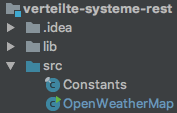
\includegraphics[width=0.2 \linewidth]{images/struktur_rest}
	\caption{Ordnerstruktur} \label{ordner}
\end{figure} 

Nun fangen wir mit der Klasse \textit{Constants.java} an, diese ist dazu da unsere Konstanten zu speichern.

\begin{lstlisting}
final class Constants {
    static final String COUNTRYCODE = "DE";
    static final String API = "&appid=722920868a0a0266c859a174da690bc1";
}
\end{lstlisting}

Wir haben hier zwei Konstanten die wir ständig benötigen, einem einen Contrycode, diesen setzen wir auf DE, da wir nur in Deutschland nach den Städten suchen. Die API Konstante speichert unseren API-Key, da wir diesen häufiger nutzen.\\\\

Nun kommen wir zur Klasse \textit{OpenWeatherMap.java}, diese macht die eigentliche Aufgabe, diese sieht wie folgt aus. 
\begin{lstlisting}
public class OpenWeatherMap {
	...
}
\end{lstlisting}

Die erste Methode die wir benötigen ist zum machen des HTTP-Request, diese hat eine Sichtbarkeit von \textit{private}, da wir sie nur in dieser Klasse verwenden.

\begin{lstlisting}
private String sendHttpRequest(String url) {
        StringBuilder json = new StringBuilder();

        try {
            URL u = new URL(url + "&units=metric" + Constants.API);
            HttpURLConnection conn = (HttpURLConnection) u.openConnection();
            conn.setRequestMethod("GET");
            BufferedReader reader = new BufferedReader(new InputStreamReader(conn.getInputStream()));
            String output;
            while ((output = reader.readLine()) != null) {
                json.append(output);
            }
        } catch (Exception e) {
            e.printStackTrace();
        }

        return json.toString();
    }
\end{lstlisting}

Wir geben einen String zurück, dieser enthält den Response als JSON und als Parameter benötigen wir nur die URL die den Request entgegen nehmen soll. Jetzt benötigen wir eine Verbindung diese machen wir mit \textit{u.openConnection()} und setzen nun noch die Methode die wir verwenden, in unserem Fall benutzen wir \textbf{GET}. Nun benutzen wir einen BufferedReader um den Response zeilenweise zu verarbeiten. Die zeilenweise Verarbeitung machen wir hier mit einem while und fügen das einem StringBuilder an und geben diesen als String zurück.\\\\

Nun benötigen wir eine Methode um den Stadtnamen herausfinden, das benötigen wir aber nur, wenn der Benutzer mit einer Postleitzahl nachdem Wetter sucht.

\begin{lstlisting}
public String getCityName(String zip) {
        String name = null;
        String json = sendHttpRequest("http://api.openweathermap.org/data/2.5/forecast/daily?zip=" + zip + "," + Constants.COUNTYCODE + "&cnt=1");

        JsonFactory factory = new JsonFactory();
        JsonParser parser;

        try {
            parser = factory.createParser(json);

            while(!parser.isClosed()){
                JsonToken jsonToken = parser.nextToken();

                if(JsonToken.FIELD_NAME.equals(jsonToken)){
                    String fieldName = parser.getCurrentName();

                    parser.nextToken();

                    if("name".equals(fieldName)){
                        name = parser.getValueAsString();
                    }
                }
            }
        } catch (IOException e) {
            e.printStackTrace();
        }

        return name;
    }
\end{lstlisting}

Wir geben einen String zurück in dem der Name der Stadt steht. Wir senden einen HTTP-Request mit unserer privaten Request-Methode, nun bekommen wir einen JSON zurück als String. Jetzt gehen wir den JSON durch bis der \textit{fieldname} gleich dem Feldname \textit{name} ist, dann wissen wir nämlich in der nächsten Value steht unser Name der Stadt und diesen geben wir dann zurück, dass müssen wir tun da man mit der Postleitzahl nicht nach der ID suchen kann.\\\\

Wir deklarieren als erstes nun globale Variablen die wir später benötigen.

\begin{lstlisting}

\end{lstlisting}

Wir schreiben jetzt eine Methode um die höchst und tiefst Temperaturen auszulesen und die sogenannte City-ID.

\begin{lstlisting}
public void getTemperatureOfDay(String city) throws IllegalArgumentException {
        String json;

        if(city.matches("\\d{3,10}")) {
            city = getCityName(city);
        }

        if(city.matches("[a-zA-ZäÄöÖüÜß]{3,}")) {
            json = sendHttpRequest("http://api.openweathermap.org/data/2.5/forecast/daily?q=" + city + "," + Constants.COUNTYCODE + "&cnt=1");
        } else {
            throw new IllegalArgumentException("wrong zip-code or city name");
        }

        JsonFactory factory = new JsonFactory();
        JsonParser parser;
        boolean idFound = false;

        try {
            parser = factory.createParser(json);

            while(!parser.isClosed()){
                JsonToken jsonToken = parser.nextToken();

                if(JsonToken.FIELD_NAME.equals(jsonToken)){
                    String fieldName = parser.getCurrentName();

                    parser.nextToken();

                    if("max".equals(fieldName)){
                        this.tx = parser.getDoubleValue();
                    } else if("min".equals(fieldName)) {
                        this.tn = parser.getDoubleValue();
                    } else if("id".equals(fieldName) && !idFound) {
                        this.cityid = parser.getValueAsInt();
                        idFound = true;
                    }
                }
            }
        } catch (IOException e) {
            e.printStackTrace();
        }
    }
\end{lstlisting}

Wir beginnen hier mit der Feststellung ob das übergebene ein Stadtname oder eine Postleitzahl ist, wenn es eine Postleitzahl ist finden wir mit unserer gerade geschriebenen Methode den Stadtnamen heraus. Nun machen wir das selbe wie eben nur suchen wir nach den Feldern \textit{max}, \textit{min} und nach der ersten \textit{id} die wir finden.\\\\

Jetzt brauchen wir noch eine Methode um die Temperaturen über den ganzen Tag zu holen.

\begin{lstlisting}
public void getHourlyTemps() {
        String json = sendHttpRequest("http://api.openweathermap.org/data/2.5/forecast?id=" + this.cityid + "&cnt=8");

        JsonFactory factory = new JsonFactory();
        JsonParser parser;

        try {
            parser = factory.createParser(json);

            String temp = "";
            String date = "";
            while (!parser.isClosed()) {
                JsonToken jsonToken = parser.nextToken();

                if (JsonToken.FIELD_NAME.equals(jsonToken)) {
                    String fieldName = parser.getCurrentName();

                    parser.nextToken();

                    if ("temp".equals(fieldName)) {
                        temp = parser.getValueAsString();
                        date = "";
                    } else if ("dt_txt".equals(fieldName)) {
                        date = parser.getValueAsString();
                    }

                    if (temp.length() > 0 && date.length() > 0) {
                        this.temps.add(date);
                        this.temps.add(temp);
                        temp = "";
                        date = "";
                    }
                }
            }
        } catch (IOException e) {
            e.printStackTrace();
        }
    }
\end{lstlisting}

Hier gehen wir ein neuen Request durch wo wir die Temperaturen von jeder Stunde bekommen und fügen für jeden Fieldname, der \textit{temp} ist das Datum von der Temperatur und die eigentliche Temperatur zu einer ArrayList hinzu, aber nur für 8 Zeilen. \\\\

Nun benötigen wir nur noch eine Methode um die Temperaturen an bestimmten Zeiten auszugeben.

\begin{lstlisting}
public void printTemps() {
        List<String> hours = Arrays.asList("06", "12", "18", "00");

        System.out.println("Datum                    |      Temperatur");

        for(int i = 0; i < temps.size(); i += 2) {
            if(hours.contains(temps.get(i).split("[ :]")[1]))
                System.out.println(temps.get(i) + "      |      " + temps.get(i+1) + " Celsius" );
        }
    }
\end{lstlisting}

Hier benutzen wir eine List da diese eine Methode zum vergleichen bietet, nun gehen wir einfach die komplette ArrayList durch und gucken ob die Zeit die gerade ist, in unserem vorher festgelegten Array ist.\\\\

Zu guter Letzt benötigen wir noch ein main damit wir das ganze Ausführen können.

\begin{lstlisting}
public static void main(String[] args) {
        OpenWeatherMap o1 = new OpenWeatherMap("32469");

        System.out.println("Minimale Temperatur: " + o1.getTn() + " Celsius\nMaximale Temperatur: " + o1.getTx() + " Celsius");

        o1.getHourlyTemps();
        o1.printTemps();
    }
\end{lstlisting} 

Wir instaziieren ein Objekt von der eben erstellten Klasse und holen uns mit zwei Get-Methoden die maximale und minimale Temperatur des Tages. Wir rufen noch die zwei geschriebenen Methoden auf.

\subsection{Fazit}
Die Aufgabe war nicht schwer zu lösen, nur konnten wir es nicht erreichen, dass wir die gewollten Zeiten von der API bekommen.